\documentclass{beamer}

% Configuracao do Latex
%\usepackage{subfiles}
\usepackage[utf8]{inputenc}
\usepackage[brazilian]{babel}
\usepackage[T1]{fontenc}
\usepackage{palatino}
\usepackage{booktabs,caption,subfigure,float}
\usepackage{graphicx,grffile}
\graphicspath{ {./img/} { ../img/ } {../../img/} {../Relatorio/img/}}

\usetheme{Hannover}

\begin{document}

\title{Indicadores Econômicos Brasileiros}
\author{Rafael Moraes}
\date{\today}

\begin{frame}
\titlepage
\end{frame}

\begin{frame}
\frametitle{Índice}\tableofcontents
\end{frame}

\section{Câmbio}
\begin{frame}
  \frametitle{Câmbio}
  \begin{figure}[ht]
    %\begin{minipage}{0.70\textheight}
      \centering
      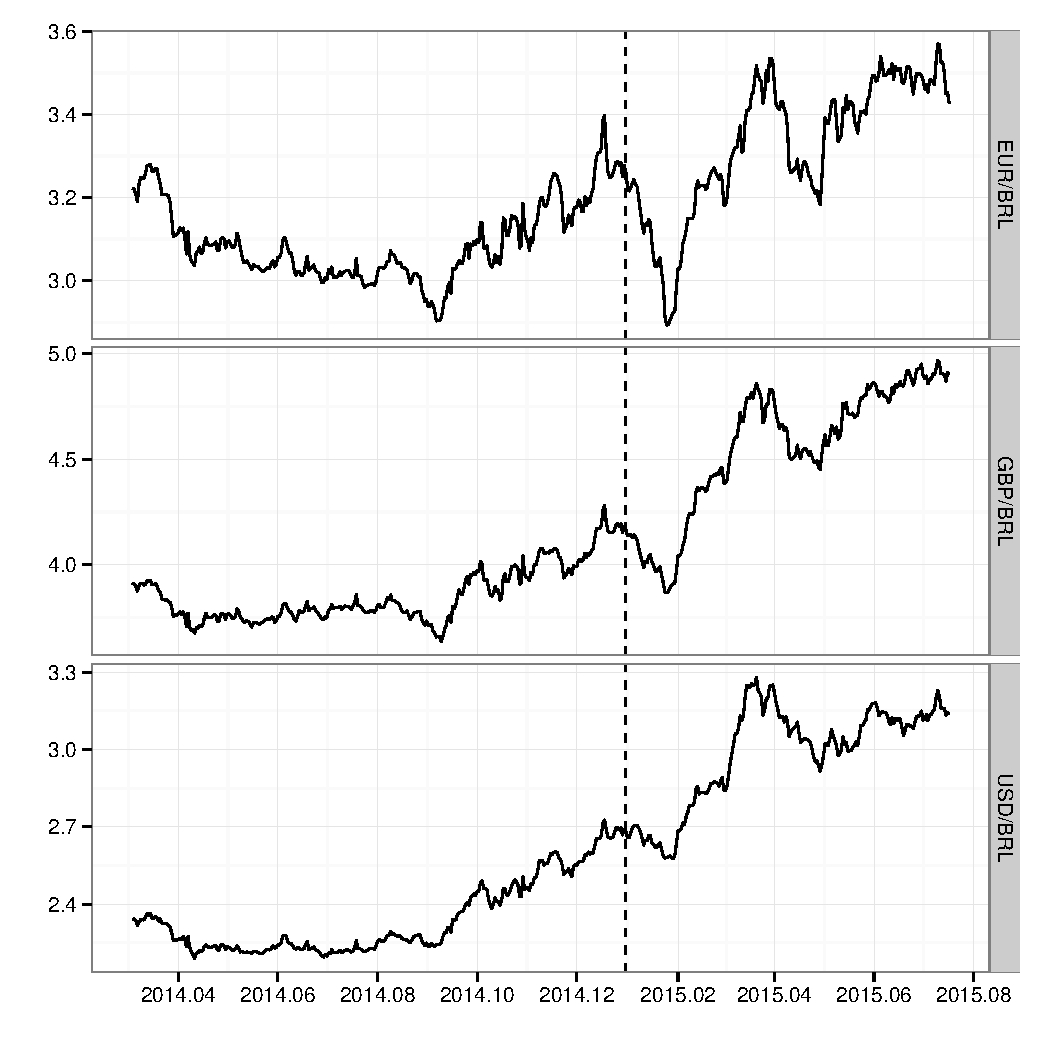
\includegraphics[height=0.80\textheight]{cambio.pdf}
    %\end{minipage}
  \end{figure}
\end{frame}

\section{Inflaçao}
\begin{frame}
  \frametitle{Inflaçao}
  \begin{figure}[ht]
    %\begin{minipage}{0.90\textheight}
      \centering
      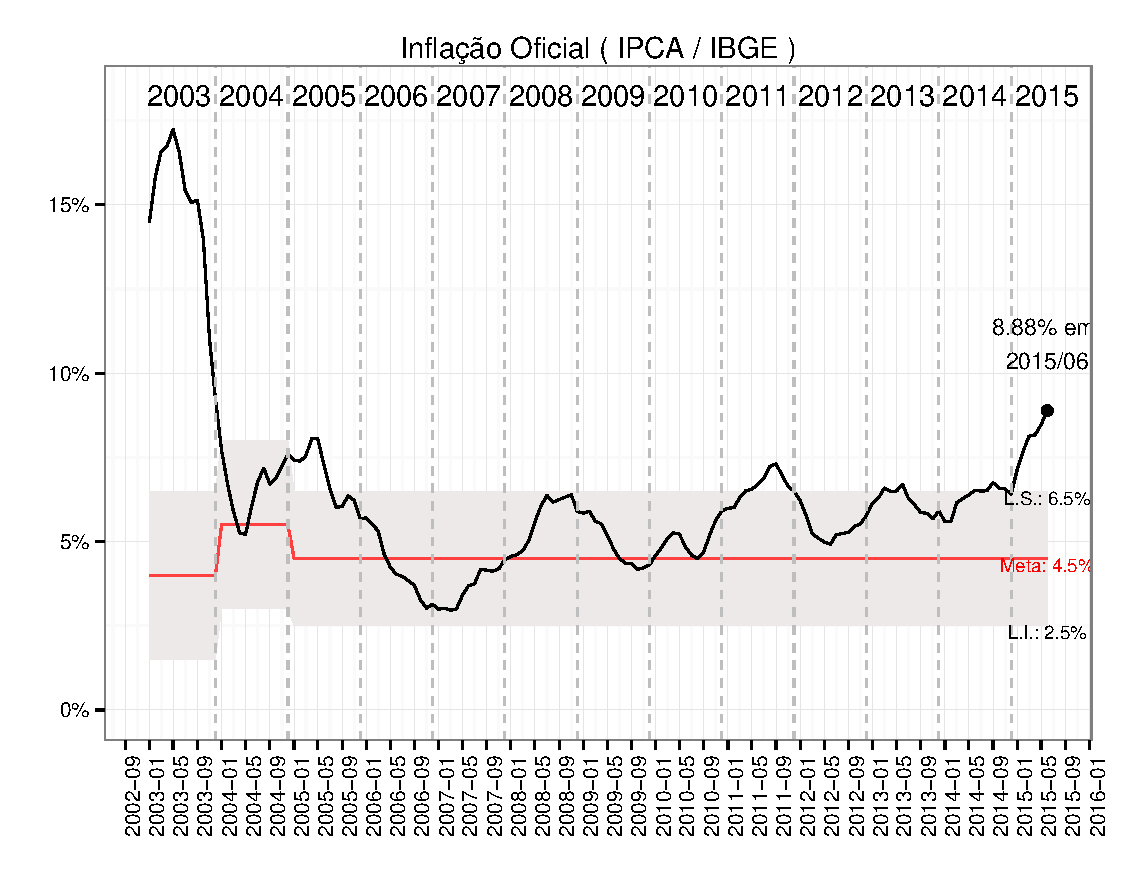
\includegraphics[width=1.00\textwidth]{Inflacao.pdf}
    %\end{minipage}
  \end{figure}
\end{frame}


\begin{frame}
  \frametitle{Inflaçao - Versao Atirei}
  \begin{figure}[ht]
    %\begin{minipage}{0.90\textheight}
      \centering
    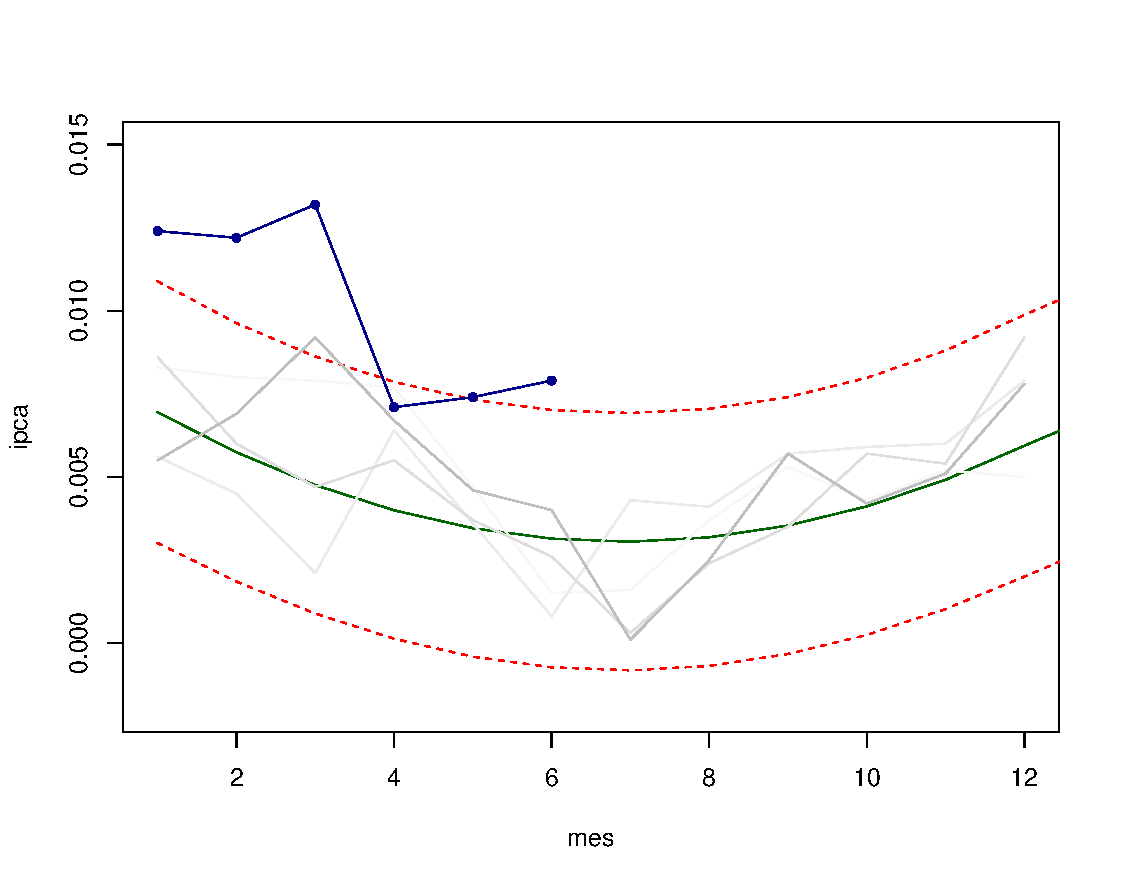
\includegraphics[width=1.00\textwidth]{IPCAatirei.pdf}
    %\end{minipage}
  \end{figure}
\end{frame}

\end{document}